\chapter{Fonctions de deux variables réelles}

\minitoc

Dans tout le chapitre, on note \(\norme{\cdot}\) la norme euclidienne canonique de \(\R^2\), \cad la norme associée au produit scalaire canonique \(\ps{\cdot}{\cdot}\) de \(\R^2\) : \[\quantifs{\forall x,y\in\R^2}\norme{\paren{x,y}}=\sqrt{x^2+y^2}.\]

\section{Ouverts de \(\R^2\)}

\begin{defi}[Boules]
Soient \(a=\paren{a_1,a_2}\in\R^2\) et \(r\in\Rp\).

La boule ouverte de centre \(a\) et de rayon \(r\) est l'ensemble des points \(x\) dont la distance à \(a\) est strictement inférieure à \(r\) : \[\bouleo{a}{r}=\accol{x\in\R^2\tq\norme{a-x}<r}.\]

La boule fermée de centre \(a\) et de rayon \(r\) est l'ensemble des points \(x\) dont la distance à \(a\) est inférieure à \(r\) : \[\boulef{a}{r}=\accol{x\in\R^2\tq\norme{a-x}\leq r}.\]

La sphère de centre \(a\) et de rayon \(r\) est l'ensemble des points \(x\) dont la distance à \(a\) est égale à \(r\) : \[\sphere{a}{r}=\accol{x\in\R^2\tq\norme{a-x}=r}.\]

Les notations \(\bouleo{a}{r}\), \(\boulef{a}{r}\) et \(\sphere{a}{r}\) ne sont pas \guillemets{officielles}.
\end{defi}

\begin{defi}
Soient \(a\in\R^2\) et \(V\subset\R^2\).

On dit que \(V\) est un voisinage de \(a\) dans \(\R^2\) s'il contient une boule centrée en \(a\) et de rayon strictement positif : \[\quantifs{\exists\epsilon\in\Rps}\bouleo{a}{\epsilon}\subset V.\]
\end{defi}

\begin{defi}[Ouvert]
Soit \(\Omega\subset\R^2\).

On dit que \(\Omega\) est un ouvert de \(\R^2\) (ou une partie ouverte de \(\R^2\)) si \(\Omega\) est un voisinage de chacun de ses points, \cad : \[\quantifs{\forall a\in\Omega;\exists\epsilon\in\Rps}\bouleo{a}{\epsilon}\subset\Omega.\]
\end{defi}

\begin{exoex}
Parmi les parties de \(\R^2\) suivantes, lesquelles sont des ouverts ?

\[\ensvide\qquad\R^2\qquad\paren{\Rps}^2\qquad\paren{\Rp}^2\qquad\R^2\excluant\accol{\paren{0,0}}\qquad\paren{\Rs}^2\qquad\intervei{0}{1}\times\R\qquad\intervee{0}{1}\times\R\]
\end{exoex}

\begin{corr}
\(\ensvide\) est un ouvert.

\(\R^2\) est un ouvert car \(\quantifs{\forall a\in\R^2}\bouleo{a}{1}\subset\R^2\).

\(\paren{\Rps}^2\) est un ouvert car \(\quantifs{\forall\paren{x,y}\in\R^2}\bouleo{\paren{x,y}}{\min\accol{\abs{x};\abs{y}}}\subset\paren{\Rps}^2\).

\(\paren{\Rp}^2\) n'est pas un ouvert.

\(\R^2\excluant\accol{\paren{0,0}}\) est un ouvert car \(\quantifs{\forall a\in\R^2\excluant\accol{\paren{0,0}}}\bouleo{a}{\norme{a}}\subset\R^2\excluant\accol{\paren{0,0}}\).

\(\paren{\Rs}^2\) est un ouvert.

\(\intervei{0}{1}\times\R\) n'est pas un ouvert.

\(\intervee{0}{1}\times\R\) est un ouvert.
\end{corr}

\section{Continuité}

Le graphe de \(f:\Omega\to\R\) où \(\Omega\) est un ouvert de \(\R^2\) est l'ensemble : \[\accol{\paren{x,y,z}\in\Omega\times\R\tq z=f\paren{x,y}}\subset\R^3.\]

Par exemple :

\begin{center}
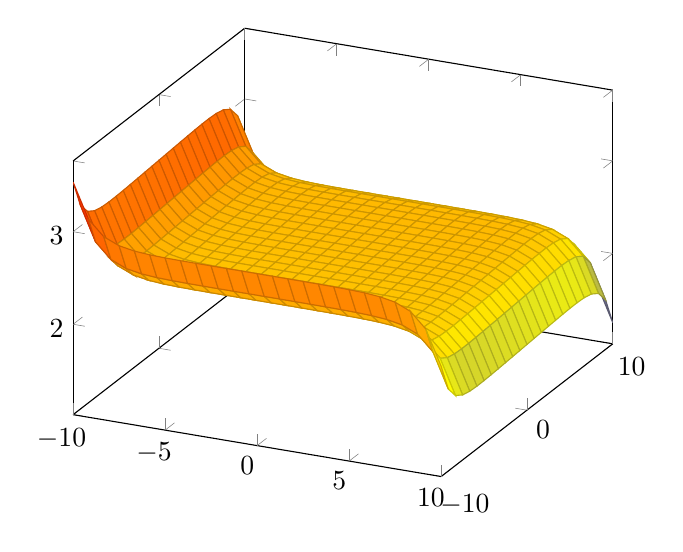
\begin{tikzpicture}
\begin{axis}
\addplot3[surf, domain=-10:10, y domain=-10:10]{0.4*cos(x)+0.4*sin(y)-0.00006*sinh(x)-0.00005*sinh(y)+2};
\end{axis}
\end{tikzpicture}
\end{center}

\begin{defi}[Fonction continue sur un ouvert de \(\R^2\)]
Soient \(\Omega\) un ouvert de \(\R^2\), \(f:\Omega\to\R\) et \(a\in\Omega\).

On dit que \(f\) est continue en \(a\) si on a : \[\quantifs{\forall\epsilon\in\Rps;\exists\delta\in\Rps;\forall x\in\Omega}\norme{x-a}\leq\delta\imp\abs{f\paren{x}-f\paren{a}}\leq\epsilon,\] \cad : \[\quantifs{\forall\epsilon\in\Rps;\exists\delta\in\Rps}f\paren{\Omega\inter\boulef{a}{\delta}}\subset\intervii{f\paren{a}-\epsilon}{f\paren{a}+\epsilon},\] \cad : \[\quantifs{\forall\epsilon\in\Rps;\exists\delta\in\Rps}\begin{dcases}
\boulef{a}{\delta}\subset\Omega \\
f\paren{\boulef{a}{\delta}}\subset\intervii{f\paren{a}-\epsilon}{f\paren{a}+\epsilon}
\end{dcases}\]

On dit que \(f\) est continue si elle est continue en tout de \(\Omega\).
\end{defi}

\begin{prop}
Soit \(\Omega\) un ouvert de \(\R^2\).

L'ensemble \(\ensclasse{0}{\Omega}{\R}\) des fonctions continues de \(\Omega\) dans \(\R\) est un sous-anneau de \(\F{\Omega}{\R}\).

Si \(f:\Omega\to\R\) et \(g:\Im f\to\R\) sont des fonctions continues alors \(g\rond f:\Omega\to\R\) est continue.

Si \(f:\Omega\to\R\) est continue alors l'ensemble \[\Omega\prim=f\inv\paren{\Rs}=\accol{x\in\Omega\tq f\paren{x}\not=0}\] est un ouvert de \(\R^2\) et la fonction \[\fonction{\dfrac{1}{f}}{\Omega\prim}{\R}{x}{\dfrac{1}{f\paren{x}}}\] est continue.
\end{prop}

\begin{dem}
\note{Exercice}
\end{dem}

\begin{exoex}
On pose : \[f:\paren{x,y}\mapsto x\qquad\text{et}\qquad g:\paren{x,y}\mapsto\Arctan\dfrac{y}{x}.\]

Pour chacune de ces fonctions, donner son ensemble de définition, dire si c'est un ouvert de \(\R^2\) et dire si la fonction est continue.
\end{exoex}

\begin{corr}
\(f\) est définie sur \(\R^2\) qui est un ouvert de \(\R^2\).

Soit \(\paren{a,b}\in\R^2\). Montrons que \(f\) est continue en \(\paren{a,b}\).

On a : \[\begin{aligned}
\quantifs{\forall\paren{x,y}\in\R^2}\abs{f\paren{x,y}-f\paren{a,b}}&=\abs{x-a} \\
&=\sqrt{\paren{x-a}^2} \\
&\leq\sqrt{\paren{x-a}^2+\paren{y-b}^2} \\
&=\norme{\paren{x,y}-\paren{a,b}}.
\end{aligned}\]

On a donc : \[\quantifs{\forall\epsilon\in\Rps;\exists\delta\in\Rps;\forall\paren{x,y}\in\R^2}\norme{\paren{x,y}-\paren{a,b}}\leq\delta\imp\abs{f\paren{x,y}-f\paren{a,b}}\leq\epsilon\] car \(\delta=\epsilon\) convient.

Donc \(f\) est continue.

\(g\) est définie sur \(\Rs\times\R\) qui est un ouvert de \(\R^2\).

De même que précédemment, \(\paren{x,y}\mapsto y\) est continue.

Donc \(\paren{x,y}\mapsto\dfrac{y}{x}\) est continue sur \(\Rs\times\R\).

Or \(\Arctan:\R\to\R\) est continue donc \(g\) est continue par composition.
\end{corr}

\section{Fonctions de classe \(\classe{1}\)}

\subsection{Développement limité d'ordre 1}

\begin{nota}
Soient \(\Omega\) un ouvert de \(\R^2\) contenant \(\paren{0,0}\) et \(g:\Omega\to\R\).

On dit que \(g\paren{x}\) est négligeable devant \(\norme{x}\) et on note \(g\paren{x}\egqd{x\to\paren{0,0}}o\paren{\norme{x}}\) si on a : \[\quantifs{\forall\epsilon\in\Rps;\exists\delta\in\Rps;\forall x\in\Omega}\norme{x}\leq\delta\imp\abs{g\paren{x}}\leq\epsilon\norme{x}.\]
\end{nota}

\begin{defi}
Soient \(\Omega\) un ouvert de \(\R^2\), \(f:\Omega\to\R\) et \(a=\paren{a_1,a_2}\in\Omega\).

On dit que \(f\) admet un développement limité à l'ordre 1 en \(a\) s'il existe \(\lambda,\mu\in\R\) tels que : \[f\paren{a_1+h_1,a_2+h_2}\egqd{h=\paren{h_1,h_2}\to\paren{0,0}}f\paren{a_1,a_2}+\lambda h_1+\mu h_2+o\paren{\norme{h}}.\]

Les réels \(\lambda\) et \(\mu\) sont alors uniques.
\end{defi}

\subsection{Dérivées partielles}

\begin{defi}
Soient \(\Omega\) un ouvert de \(\R^2\), \(f:\Omega\to\R\) et \(a=\paren{a_1,a_2}\in\Omega\).

On dit que \(f\) admet une dérivée partielle par rapport à \(x\) en \(a\) si la fonction \(\gamma:t\mapsto f\paren{t,a_2}\) est dérivable en \(a_1\).

On pose alors : \[\pdv{f}{x}\paren{a}=\gamma\prim\paren{a_1}.\]

On définit de même \(\pdv{f}{y}\).
\end{defi}


\begin{exoex}
Calculer les dérivées partielles de \[f:\paren{x,y}\mapsto x^3y^2+x+1\qquad\text{et}\qquad g:\paren{x,y}\mapsto\Arctan\dfrac{y}{x}.\]
\end{exoex}


\begin{corr}
On a : \[\quantifs{\forall\paren{x,y}\in\R^2}\begin{dcases}
\pdv{f}{x}\paren{x,y}=3x^2y^2+1 \\
\pdv{f}{y}\paren{x,y}=2x^3y
\end{dcases}\] et : \[\quantifs{\forall\paren{x,y}\in\Rs\times\R}\begin{dcases}
\pdv{g}{x}\paren{x,y}=\dfrac{-y}{x^2}\times\dfrac{1}{1+\paren{\frac{y}{x}}^2}=\dfrac{-y}{x^2+y^2} \\
\pdv{g}{y}\paren{x,y}=\dfrac{1}{x}\times\dfrac{1}{1+\paren{\frac{y}{x}}^2}=\dfrac{x}{x^2+y^2}
\end{dcases}\]
\end{corr}


\begin{rem}
Soient \(\Omega\) un ouvert de \(\R^2\), \(f:\Omega\to\R\) et \(a\in\Omega\).

Le fait que \(f\) admette des dérivées partielles en \(a\) n'implique pas la continuité de \(f\) en \(a\).
\end{rem}

\subsection{Fonctions de classe \(\classe{1}\)}


\begin{defi}
Soit \(\Omega\) un ouvert de \(\R^2\).

On dit qu'une fonction \(f:\Omega\to\R\) est de classe \(\classe{1}\) si ses dérivées partielles \(\pdv{f}{x}\) et \(\pdv{f}{y}\) sont définies et continues.
\end{defi}


\begin{theo}
Soient \(\Omega\) un ouvert de \(\R^2\) et \(f:\Omega\to\R\) de classe \(\classe{1}\).

Alors \(f\) admet un développement limité à l'ordre 1 en tout point de \(\Omega\).

Soit \(\paren{x_0,y_0}\in\Omega\).

Alors on a : \[f\paren{x_1,y_1}\egqd{\paren{x_1,y_1}\to\paren{x_0,y_0}}f\paren{x_0,y_0}+\paren{x_1-x_0}\pdv{f}{x}\paren{x_0,y_0}+\paren{y_1-y_0}\pdv{f}{y}\paren{x_0,y_0}+o\paren{\norme{\paren{x_1-x_0,y_1-y_0}}}\]
\end{theo}

\begin{dem}
On a : \[\begin{aligned}
f\paren{x_1,y_1}-f\paren{x_0,y_0}&=f\paren{x_1,y_1}-f\paren{x_1,y_0}+f\paren{x_1,y_0}-f\paren{x_0,y_0} \\
&=\int_{y_0}^{y_1}\pdv{f}{y}\paren{x_1,t}\odif{t}+\int_{x_0}^{x_1}\pdv{f}{x}\paren{t,y_0}\odif{t} \\
&=\int_{y_0}^{y_1}\paren{\pdv{f}{y}\paren{x_1,t}-\pdv{f}{y}\paren{x_0,y_0}}\odif{t}+\int_{y_0}^{y_1}\pdv{f}{y}\paren{x_0,y_0}\odif{t} \\
&\color{white}=\color{black}+\int_{x_0}^{x_1}\paren{\pdv{f}{x}\paren{t,y_0}-\pdv{f}{x}\paren{x_0,y_0}}\odif{t}+\int_{x_0}^{x_1}\pdv{f}{x}\paren{x_0,y_0}\odif{t}
\end{aligned}\]

Soient \(\epsilon,\delta\in\Rps\) tels que \(\begin{dcases}
\bouleo{\paren{x_0,y_0}}{\delta}\subset\Omega \\
\quantifs{\forall a\in\bouleo{\paren{x_0,y_0}}{\delta}}\begin{dcases}
\abs{\pdv{f}{x}\paren{a}-\pdv{f}{x}\paren{x_0,y_0}}\leq\epsilon \\
\abs{\pdv{f}{y}\paren{a}-\pdv{f}{y}\paren{x_0,y_0}}\leq\epsilon
\end{dcases}
\end{dcases}\)

On a : \[\begin{aligned}
f\paren{x_1,y_1}-f\paren{x_0,y_0}&=\underbrace{\int_{y_0}^{y_1}\underbrace{\paren{\pdv{f}{y}\paren{x_1,t}-\pdv{f}{y}\paren{x_0,y_0}}}_{\abs{\cdot}\leq\epsilon}\odif{t}}_{\leq\abs{y_1-y_0}\epsilon}+\underbrace{\int_{y_0}^{y_1}\pdv{f}{y}\paren{x_0,y_0}\odif{t}}_{=\paren{y_1-y_0}\pdv{f}{y}\paren{x_0,y_0}} \\
&\color{white}=\color{black}+\underbrace{\int_{x_0}^{x_1}\underbrace{\paren{\pdv{f}{x}\paren{t,y_0}-\pdv{f}{x}\paren{x_0,y_0}}}_{\abs{\cdot}\leq\epsilon}\odif{t}}_{\leq\abs{x_1-x_0}\epsilon}+\underbrace{\int_{x_0}^{x_1}\pdv{f}{x}\paren{x_0,y_0}\odif{t}}_{=\paren{x_1-x_0}\pdv{f}{x}\paren{x_0,y_0}}
\end{aligned}\]

Donc \[\begin{aligned}
\int_{y_0}^{y_1}\paren{\pdv{f}{y}\paren{x_1,t}-\pdv{f}{y}\paren{x_0,y_0}}\odif{t}+\int_{x_0}^{x_1}\paren{\pdv{f}{x}\paren{t,y_0}-\pdv{f}{x}\paren{x_0,y_0}}\odif{t}&\leq2\epsilon\norme{\paren{x_1,y_1}-\paren{x_0,y_0}} \\
&=o\paren{\norme{\paren{x_1-x_0,y_1-y_0}}}.
\end{aligned}\]

D'où le résultat.
\end{dem}

\begin{defi}[Gradient]
Soient \(\Omega\) un ouvert de \(\R^2\), \(f\in\ensclasse{1}{\Omega}{\R}\) et \(a\in\Omega\).

On appelle gradient de \(f\) en \(a\) le vecteur \[\nabla f\paren{a}=\paren{\pdv{f}{x}\paren{a},\pdv{f}{y}\paren{a}}.\]

Selon le théorème précédent, il vérifie : \[f\paren{a+h}\egqd{h\to\paren{0,0}}f\paren{a}+\ps{\nabla f\paren{a}}{h}+o\paren{\norme{h}}.\]
\end{defi}

\begin{exoex}
Calculer le gradient des fonctions \[\fonction{f}{\R^2\excluant\accol{\paren{0,0}}}{\R}{\paren{x,y}}{\sqrt{x^2+y^2}}\qquad\text{et}\qquad\fonction{g}{\Rps\times\R}{\R}{\paren{x,y}}{\Arctan\dfrac{y}{x}}\]
\end{exoex}

\begin{corr}
On a : \[\quantifs{\forall\paren{x,y}\in\R^2\excluant\accol{\paren{0,0}}}\nabla f\paren{x,y}=\paren{\dfrac{x}{\sqrt{x^2+y^2}},\dfrac{y}{\sqrt{x^2+y^2}}}=\dfrac{1}{\sqrt{x^2+y^2}}\paren{x,y}\] et : \[\quantifs{\forall\paren{x,y}\in\Rps\times\R}\nabla g\paren{x,y}=\paren{\dfrac{-y}{x^2+y^2},\dfrac{x}{x^2+y^2}}=\dfrac{1}{x^2+y^2}\paren{-y,x}.\]
\end{corr}

\subsection{Règle de la chaîne}

\begin{prop}
Soient \(\Omega\) un ouvert de \(\R^2\), \(f\in\ensclasse{1}{\Omega}{\R}\) et \(I\) un intervalle de \(\R\) tel que \(\Card I\geq2\).

Soit \(\fonction{\gamma}{I}{\Omega}{t}{\paren{\gamma_1\paren{t},\gamma_2\paren{t}}}\)

On suppose que \(\gamma_1\) et \(\gamma_2\) sont de classe \(\classe{1}\).

Alors \(\fonction{g}{I}{\R}{t}{f\paren{\gamma\paren{t}}}\) est de classe \(\classe{1}\) et sa dérivée est : \[\quantifs{\forall t\in I}g\prim\paren{t}=\pdv{f}{x}\paren{\gamma\paren{t}}\gamma_1\prim\paren{t}+\pdv{f}{y}\paren{\gamma\paren{t}}\gamma_2\prim\paren{t}.\]
\end{prop}

\begin{dem}
Soit \(t\in I\).

On a, quand \(h\to0\) : \(\begin{dcases}
\gamma_1\paren{t+h}=\gamma_1\paren{t}+\gamma_1\prim\paren{t}h+o\paren{h} \\
\gamma_2\paren{t+h}=\gamma_2\paren{t}+\gamma_2\prim\paren{t}h+o\paren{h}
\end{dcases}\)

Donc : \[\begin{aligned}
g\paren{t+h}&=f\paren{\gamma_1\paren{t}+\underbrace{\gamma_1\prim\paren{t}h+o\paren{h}}_{\to0},\gamma_2\paren{t}+\underbrace{\gamma_2\prim\paren{t}h+o\paren{h}}_{\to0}} \\
&=f\paren{\gamma\paren{t}}+\pdv{f}{x}\paren{\gamma\paren{t}}\paren{\gamma_1\prim\paren{t}h+o\paren{h}}+\pdv{f}{y}\paren{\gamma\paren{t}}\paren{\gamma_2\prim\paren{t}h+o\paren{h}} \\
&\color{white}=\color{black}+\underbrace{o\paren{\norme{\paren{\underbrace{\gamma_1\prim\paren{t}h+o\paren{h}}_{O\paren{h}},\underbrace{\gamma_2\prim\paren{t}h+o\paren{h}}_{O\paren{h}}}}}}_{o\paren{h}} \\
&=g\paren{t}+\paren{\pdv{f}{x}\paren{\gamma\paren{t}}\gamma_1\prim\paren{t}+\pdv{f}{y}\paren{\gamma\paren{t}}\gamma_2\prim\paren{t}}h+o\paren{h}
\end{aligned}\]

Donc \(g\) est dérivable, de dérivée \(\pdv{f}{x}\paren{\gamma\paren{t}}\gamma_1\prim\paren{t}+\pdv{f}{y}\paren{\gamma\paren{t}}\gamma_2\prim\paren{t}\).
\end{dem}

\begin{defprop}[Dérivée selon un vecteur]
Soient \(\Omega\) un ouvert de \(\R^2\), \(f:\Omega\to\R\), \(a\in\Omega\) et \(v\in\R^2\).

On appelle dérivée de \(f\) en \(a\) selon \(v\) la dérivée en \(0\) (si elle existe) de \(t\mapsto f\paren{a+tv}\).

On la note \(\vdv{v}{f}\paren{a}\).

Si \(f\) est de classe \(\classe{1}\) alors \(\vdv{v}{f}\paren{a}\) existe et vaut \[\vdv{v}{f}\paren{a}=\ps{\nabla f\paren{a}}{v}.\]
\end{defprop}

\begin{dem}
Notons \(v=\paren{v_1,v_2}\).

On a, pour tout \(t\) suffisamment petit : \[f\paren{a+tv}=f\paren{a_1+tv_1,a_2+tv_2}.\]

Donc selon la règle de la chaîne : \[\begin{aligned}
\vdv{v}{f}\paren{a}&=v_1\pdv{f}{x}\paren{a}+v_2\pdv{f}{y}\paren{a} \\
&=\ps{\dcoords{v_1}{v_2}}{\nabla f\paren{a}}.
\end{aligned}\]
\end{dem}

\begin{cor}
Soient \(\Omega,\Omega\prim\) deux ouverts de \(\R^2\), \(f\in\ensclasse{1}{\Omega}{\R}\) et \(\phi,\psi\in\ensclasse{1}{\Omega\prim}{\R}\).

On suppose \(\quantifs{\forall u,v\in\Omega\prim}\paren{\phi\paren{u,v},\psi\paren{u,v}}\in\Omega\).

On pose \(\fonction{g}{\Omega\prim}{\R}{\paren{u,v}}{f\paren{\phi\paren{u,v},\psi\paren{u,v}}}\)

Alors \(g\) est de classe \(\classe{1}\) et on a : \[\quantifs{\forall a\in\Omega\prim}\begin{dcases}
\pdv{g}{u}\paren{a}=\pdv{f}{x}\paren{\phi\paren{a},\psi\paren{a}}\pdv{\phi}{u}\paren{u,v}+\pdv{f}{y}\paren{\phi\paren{a},\psi\paren{a}}\pdv{\psi}{u}\paren{u,v} \\
\pdv{g}{v}\paren{a}=\pdv{f}{x}\paren{\phi\paren{a},\psi\paren{a}}\pdv{\phi}{v}\paren{u,v}+\pdv{f}{v}\paren{\phi\paren{a},\psi\paren{a}}\pdv{\psi}{v}\paren{u,v}
\end{dcases}\]
\end{cor}

\subsection{Équations aux dérivées partielles}

\begin{ex}
Résolvons sur \(\R^2\) l'équation aux dérivées partielles \(\paren{E}~\pdv{f}{x}\paren{x,y}=x^2y^2\).

Soit \(f\in\ensclasse{1}{\R^2}{\R}\).

On a : \[f\text{ est solution de }\paren{E}\ssi\quantifs{\exists g\in\ensclasse{1}{\R}{\R};\forall\paren{x,y}\in\R^2}f\paren{x,y}=\dfrac{1}{3}x^3y^2+g\paren{y}.\]
\end{ex}

\begin{ex}
Résolvons sur \(\R^2\) l'équation aux dérivées partielles \(\paren{E}~\pdv[order=2]{f}{x}\paren{x,y}=\cos x+\sin y+\exp\paren{x\e{y}}\).

Soit \(f\in\ensclasse{2}{\R^2}{\R}\) (\cad \(\pdv{f}{x},\pdv{f}{y}\in\ensclasse{1}{\R^2}{\R}\)).

On a : \[\begin{aligned}
f\text{ est solution de }\paren{E}&\ssi\quantifs{\exists g\in\F{\R}{\R};\forall\paren{x,y}\in\R^2}\pdv{f}{x}\paren{x,y}=\sin x+x\sin y \\
&\color{white}\ssi\quantifs{\exists g\in\F{\R}{\R};\forall\paren{x,y}\in\R^2}\pdv{f}{x}\paren{x,y}=\color{black}+\e{-y}\exp\paren{x\e{y}}+g\paren{y} \\
&\ssi\quantifs{\exists g,h\in\F{\R}{\R};\forall\paren{x,y}\in\R^2}f\paren{x,y}=-\cos x+\dfrac{1}{2}x^2\sin y \\
&\color{white}\ssi\quantifs{\exists g,h\in\F{\R}{\R};\forall\paren{x,y}\in\R^2}f\paren{x,y}=\color{black}+\e{-2y}\exp\paren{x\e{y}}+xg\paren{y}+h\paren{y}
\end{aligned}\] où \(g,h\in\ensclasse{2}{\R}{\R}\).
\end{ex}

% le cours en est là pour le moment